\hypertarget{_t89_8c}{
\section{/home/mgh/LanlGeoMag/libLanlGeoMag/T89.c File Reference}
\label{_t89_8c}\index{/home/mgh/LanlGeoMag/libLanlGeoMag/T89.c@{/home/mgh/LanlGeoMag/libLanlGeoMag/T89.c}}
}
{\tt \#include \char`\"{}Lgm/Lgm\_\-MagModelInfo.h\char`\"{}}\par


Include dependency graph for T89.c:\nopagebreak
\begin{figure}[H]
\begin{center}
\leavevmode
\includegraphics[width=291pt]{_t89_8c__incl}
\end{center}
\end{figure}
\subsection*{Functions}
\begin{CompactItemize}
\item 
int \hyperlink{_t89_8c_c837cac3ed79e2e8b7d38c84635dbad1}{Lgm\_\-BT\_\-T89} (\hyperlink{struct_lgm___vector}{Lgm\_\-Vector} $\ast$v, \hyperlink{struct_lgm___vector}{Lgm\_\-Vector} $\ast$B, \hyperlink{struct_lgm___mag_model_info}{Lgm\_\-MagModelInfo} $\ast$Info)
\item 
int \hyperlink{_t89_8c_1a66495559b8f607826fddfa540f2a25}{Lgm\_\-BRC\_\-T89} (\hyperlink{struct_lgm___vector}{Lgm\_\-Vector} $\ast$v, \hyperlink{struct_lgm___vector}{Lgm\_\-Vector} $\ast$B, \hyperlink{struct_lgm___mag_model_info}{Lgm\_\-MagModelInfo} $\ast$Info)
\item 
int \hyperlink{_t89_8c_f861a8af8bd8d861d781cffd5a21bf61}{Lgm\_\-BM\_\-T89} (\hyperlink{struct_lgm___vector}{Lgm\_\-Vector} $\ast$v, \hyperlink{struct_lgm___vector}{Lgm\_\-Vector} $\ast$B, \hyperlink{struct_lgm___mag_model_info}{Lgm\_\-MagModelInfo} $\ast$Info)
\item 
int \hyperlink{_t89_8c_7819d2e381582c64e55ea3a1c94a293e}{Lgm\_\-BC\_\-T89} (\hyperlink{struct_lgm___vector}{Lgm\_\-Vector} $\ast$v, \hyperlink{struct_lgm___vector}{Lgm\_\-Vector} $\ast$B, \hyperlink{struct_lgm___mag_model_info}{Lgm\_\-MagModelInfo} $\ast$Info)
\item 
int \hyperlink{_t89_8c_d31ae081cf3eed687888470191d52b4b}{Lgm\_\-B\_\-T89} (\hyperlink{struct_lgm___vector}{Lgm\_\-Vector} $\ast$v, \hyperlink{struct_lgm___vector}{Lgm\_\-Vector} $\ast$B, \hyperlink{struct_lgm___mag_model_info}{Lgm\_\-MagModelInfo} $\ast$Info)
\end{CompactItemize}


\subsection{Function Documentation}
\hypertarget{_t89_8c_c837cac3ed79e2e8b7d38c84635dbad1}{
\index{T89.c@{T89.c}!Lgm\_\-BT\_\-T89@{Lgm\_\-BT\_\-T89}}
\index{Lgm\_\-BT\_\-T89@{Lgm\_\-BT\_\-T89}!T89.c@{T89.c}}
\subsubsection[{Lgm\_\-BT\_\-T89}]{\setlength{\rightskip}{0pt plus 5cm}int Lgm\_\-BT\_\-T89 ({\bf Lgm\_\-Vector} $\ast$ {\em v}, \/  {\bf Lgm\_\-Vector} $\ast$ {\em B}, \/  {\bf Lgm\_\-MagModelInfo} $\ast$ {\em Info})}}
\label{_t89_8c_c837cac3ed79e2e8b7d38c84635dbad1}




Definition at line 93 of file T89.c.

Here is the caller graph for this function:\nopagebreak
\begin{figure}[H]
\begin{center}
\leavevmode
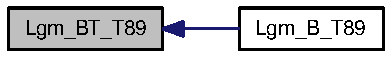
\includegraphics[width=112pt]{_t89_8c_c837cac3ed79e2e8b7d38c84635dbad1_icgraph}
\end{center}
\end{figure}
\hypertarget{_t89_8c_1a66495559b8f607826fddfa540f2a25}{
\index{T89.c@{T89.c}!Lgm\_\-BRC\_\-T89@{Lgm\_\-BRC\_\-T89}}
\index{Lgm\_\-BRC\_\-T89@{Lgm\_\-BRC\_\-T89}!T89.c@{T89.c}}
\subsubsection[{Lgm\_\-BRC\_\-T89}]{\setlength{\rightskip}{0pt plus 5cm}int Lgm\_\-BRC\_\-T89 ({\bf Lgm\_\-Vector} $\ast$ {\em v}, \/  {\bf Lgm\_\-Vector} $\ast$ {\em B}, \/  {\bf Lgm\_\-MagModelInfo} $\ast$ {\em Info})}}
\label{_t89_8c_1a66495559b8f607826fddfa540f2a25}




Definition at line 217 of file T89.c.

Here is the caller graph for this function:\nopagebreak
\begin{figure}[H]
\begin{center}
\leavevmode
\includegraphics[width=116pt]{_t89_8c_1a66495559b8f607826fddfa540f2a25_icgraph}
\end{center}
\end{figure}
\hypertarget{_t89_8c_f861a8af8bd8d861d781cffd5a21bf61}{
\index{T89.c@{T89.c}!Lgm\_\-BM\_\-T89@{Lgm\_\-BM\_\-T89}}
\index{Lgm\_\-BM\_\-T89@{Lgm\_\-BM\_\-T89}!T89.c@{T89.c}}
\subsubsection[{Lgm\_\-BM\_\-T89}]{\setlength{\rightskip}{0pt plus 5cm}int Lgm\_\-BM\_\-T89 ({\bf Lgm\_\-Vector} $\ast$ {\em v}, \/  {\bf Lgm\_\-Vector} $\ast$ {\em B}, \/  {\bf Lgm\_\-MagModelInfo} $\ast$ {\em Info})}}
\label{_t89_8c_f861a8af8bd8d861d781cffd5a21bf61}




Definition at line 322 of file T89.c.

Here is the caller graph for this function:\nopagebreak
\begin{figure}[H]
\begin{center}
\leavevmode
\includegraphics[width=114pt]{_t89_8c_f861a8af8bd8d861d781cffd5a21bf61_icgraph}
\end{center}
\end{figure}
\hypertarget{_t89_8c_7819d2e381582c64e55ea3a1c94a293e}{
\index{T89.c@{T89.c}!Lgm\_\-BC\_\-T89@{Lgm\_\-BC\_\-T89}}
\index{Lgm\_\-BC\_\-T89@{Lgm\_\-BC\_\-T89}!T89.c@{T89.c}}
\subsubsection[{Lgm\_\-BC\_\-T89}]{\setlength{\rightskip}{0pt plus 5cm}int Lgm\_\-BC\_\-T89 ({\bf Lgm\_\-Vector} $\ast$ {\em v}, \/  {\bf Lgm\_\-Vector} $\ast$ {\em B}, \/  {\bf Lgm\_\-MagModelInfo} $\ast$ {\em Info})}}
\label{_t89_8c_7819d2e381582c64e55ea3a1c94a293e}




Definition at line 348 of file T89.c.

Here is the caller graph for this function:\nopagebreak
\begin{figure}[H]
\begin{center}
\leavevmode
\includegraphics[width=113pt]{_t89_8c_7819d2e381582c64e55ea3a1c94a293e_icgraph}
\end{center}
\end{figure}
\hypertarget{_t89_8c_d31ae081cf3eed687888470191d52b4b}{
\index{T89.c@{T89.c}!Lgm\_\-B\_\-T89@{Lgm\_\-B\_\-T89}}
\index{Lgm\_\-B\_\-T89@{Lgm\_\-B\_\-T89}!T89.c@{T89.c}}
\subsubsection[{Lgm\_\-B\_\-T89}]{\setlength{\rightskip}{0pt plus 5cm}int Lgm\_\-B\_\-T89 ({\bf Lgm\_\-Vector} $\ast$ {\em v}, \/  {\bf Lgm\_\-Vector} $\ast$ {\em B}, \/  {\bf Lgm\_\-MagModelInfo} $\ast$ {\em Info})}}
\label{_t89_8c_d31ae081cf3eed687888470191d52b4b}




Definition at line 429 of file T89.c.

Here is the call graph for this function:\nopagebreak
\begin{figure}[H]
\begin{center}
\leavevmode
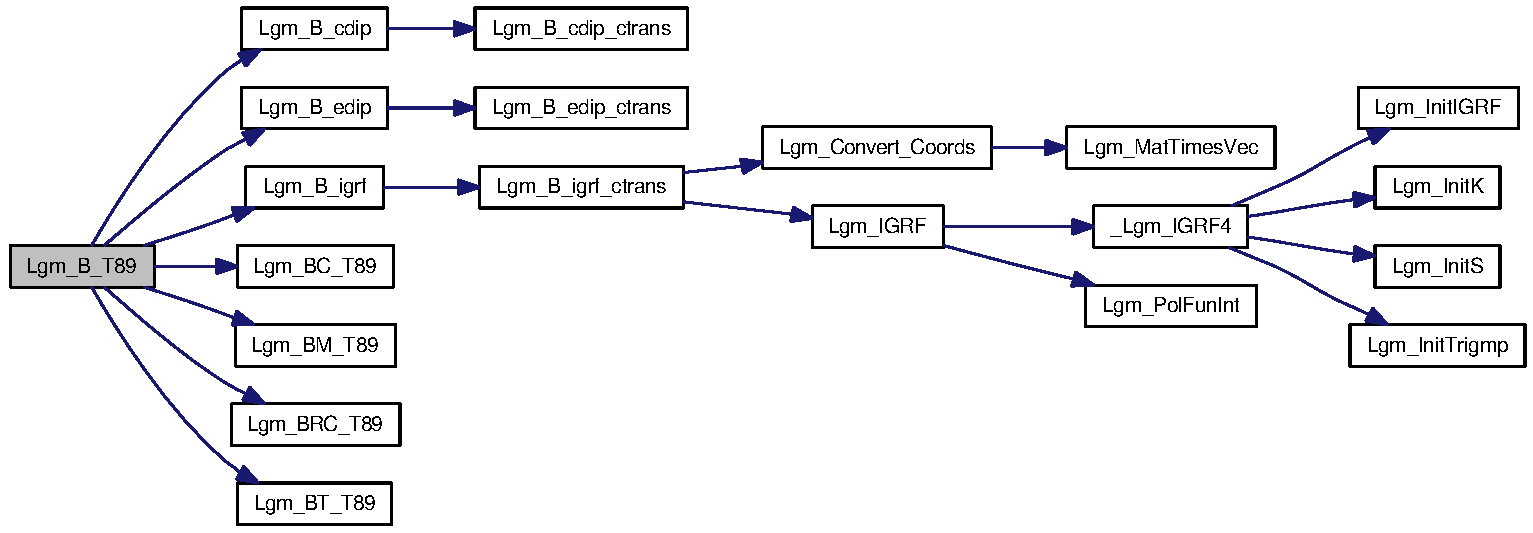
\includegraphics[width=386pt]{_t89_8c_d31ae081cf3eed687888470191d52b4b_cgraph}
\end{center}
\end{figure}
